\chapter{Working with Images}\label{ch:workingwithimages}

This chapter is designed to be a first introduction to programming
using the Vision Workbench.  It describes images, pixels, color
spaces, image file I/O, and basic image manipulation, setting the
stage for the fundamental image processing operations described in
Chapter~\ref{ch:imageprocessing}.

\section{The {\tt ImageView} Class}

The \verb#ImageView# class is the centerpiece of the Vision Workbench
in most applications.  Simply put, it represents an image in memory.
The class is similar to related classes that appear in other C++ computer
vision libraries, including VXL, GIL, and VIGRA, so if you are already
familiar with one of those libraries you should find nothing too
foreign here.

\subsection{The Basics}
An \verb#ImageView# represents a two-dimensional rectangular array of
data, such as an image of pixels.  It is actually a class {\it template},
and when you declare an \verb#ImageView# object you specify the
particular kind of data that it should contain.  For example, you can
make an \verb#ImageView# of RGB (red/green/blue) pixels to represent a
full-color image or an \verb#ImageView# of vectors to represent a vector
field.  You specify the pixel type as a template parameter to the
\verb#ImageView# class like this:
\begin{verbatim}
  ImageView<PixelRGB<float32> > my_image;
\end{verbatim}
In this case we've made a full-color RGB image.  Notice that
\verb#PixelRGB# is itself a template: here we've specified that we
want each channel of each RGB pixel to be stored as a 32-bit
floating-point number.  All of the core pixel types in the Vision
Workbench are themselves templates like this.

The \verb#ImageView# class is defined in the C++ header file
\verb#<vw/Image/ImageView.h>#, and the standard pixel types are
defined in the header \verb#<vw/Image/PixelTypes.h>#.  Thus, for the
above line of code to compile you must include those two headers at
the top of your program.  (Alternatively, all of the header files
relating to basic image manipulation are collected together in the
convenience header \verb#<vw/Image.h>#.)  Furthermore, all of the core
classes and functions of the Vision Workbench are defined in the C++
namespace \verb#vw#.  One way to use them is to be fully specific:
\begin{verbatim}
  vw::ImageView<vw::PixelRGB<vw::float32> > my_image;
\end{verbatim}
The other way, which may be simpler for new users, is to bring the
entire \verb#vw# namespace into the global scope by saying
\begin{verbatim}
  using namespace vw;
\end{verbatim}
at the top of your program after you've included the necessary
headers.  For brevity, in the examples in this book we will often
assume that you have included the necessary headers and we will omit
explicit references to namespace \verb#vw#.  The exception to this is
the complete programs, such as \verb#vwconvert.cc#
(Listing~\ref{lst:vwconvert.cc}, above), which are intended to be
fully self-contained.

By default the dimensions of an \verb#ImageView# are zero, which may not
be what you want.  One option is to specify an image's dimensions when
we construct it:
\begin{verbatim}
  ImageView<PixelRGB<float> > my_image( 320, 240 );
\end{verbatim}
This creates an image with 320 columns and 240 rows.  If we ever want to
set or change the size of an image later on in the code we can use the
\verb#set_size()# method:
\begin{verbatim}
  my_image.set_size( 640, 480 );
\end{verbatim}
You can also find out how many columns or rows an image has using the
\verb#cols()# and \verb#rows()# methods, respectively:
\begin{verbatim}
  int width = my_image.cols();
  int height = my_image.rows();
\end{verbatim}
Note that when you call \verb#set_size()# with new image dimensions
the Vision Workbench allocates a new chunk of memory of the
appropriate size.  This is a destructive operation: any old data is
not copied into the new buffer, and the old buffer will be
automatically deallocated if no other objects are using it.

Once you've made an \verb#ImageView#, the simplest way to access a
particular pixel is by indexing directly into it:
\begin{verbatim}
  PixelRGB<float> some_pixel = my_image( x, y );
\end{verbatim}
In this example we've assumed that \verb#x# and \verb#y# are integer
variables with the desired pixel's coordinates.  For a less trivial
example, one way to fill our image with the color red would be to loop
over all the rows and columns, setting each pixel at a time:
\begin{verbatim}
  PixelRGB<float> red(1.0, 0.0, 0.0);
  for ( int y=0; y<my_image.rows(); ++y )
    for ( int x=0; x<my_image.cols(); ++x )
      my_image(x,y) = red;
\end{verbatim}
This is not the fastest way to access the pixels of an image, but
it is arguably the most flexible.  (Later we will learn about much
simpler ways to fill an image with a single color.)

\subsection{The Standard Pixel Types}

The Vision Workbench provides a number of standard pixel types that
you can use to manipulate the most common sorts of images.  We've
already encountered \verb#PixelRGB#, the standard RGB pixel type.  As
we mentioned earlier, this is a template class whose template
parameter specifies the underlying numeric data type used to store
each channel of the pixel.  This is called the pixel's {\it channel
  type}.  The Vision Workbench defines convenient platform-independent
names for the standard channel types, so that you never have to worry
about whether \verb#int# or \verb#short# is 16 bits wide on your
platform.  These Vision Workbench channel types are listed in
Table~\ref{tbl:channel-types}.  These are the only channel types with
which the Vision Workbench has been tested, so it is best to stick to
these unless you have a compelling reason not to.

\begin{table}[t]\begin{centering}
\begin{tabular}{|c|l|l|} \hline
Type & Description & Notes \\ \hline \hline
\verb#int8# & Signed 8-bit integer & \\ \hline
\verb#uint8# & Unsigned 8-bit integer & Common for low-dynamic-range imaging \\ \hline
\verb#int16# & Signed 16-bit integer & \\ \hline
\verb#uint16# & Unsigned 16-bit integer & \\ \hline
\verb#int32# & Signed 32-bit integer & \\ \hline
\verb#uint32# & Unsigned 32-bit integer & \\ \hline
\verb#int64# & Signed 64-bit integer & \\ \hline
\verb#uint64# & Unsigned 64-bit integer & \\ \hline
\verb#float32# & 32-bit floating point & Common for high-dynamic-range imaging \\ \hline
\verb#float64# & 64-bit floating point & \\ \hline
\end{tabular}
\caption{The standard Vision Workbench channel types.}
\label{tbl:channel-types}
\end{centering}\end{table}

\begin{table}[t]\begin{centering}
\begin{tabular}{|c|l|l|} \hline
Type & Description & Channels \\ \hline \hline
\verb#PixelGray<T># & Grayscale & Grayscale value (\verb#v#) \\ \hline
\verb#PixelGrayA<T># & Grayscale w/ alpha & Grayscale value (\verb#v#), alpha (\verb#a#) \\ \hline
\verb#PixelRGB<T># & RGB & Red (\verb#r#), green (\verb#g#), blue (\verb#b#) \\ \hline
\verb#PixelRGBA<T># & RGB w/ alpha &  Red (\verb#r#), green (\verb#g#), blue (\verb#b#), alpha (\verb#a#) \\ \hline
\verb#PixelHSV<T># & HSV & Hue (\verb#h#), saturation (\verb#s#), value (\verb#v#) \\ \hline
\verb#PixelXYZ<T># & XYZ & CIE 1931 X (\verb#x#), Y (\verb#y#), and Z (\verb#z#) channels \\ \hline
\verb#Vector<T,N># & An \verb#N#-dimensional vector & \verb#N# vector components \\ \hline
\verb#T# & A unitless scalar & N/A \\ \hline
\end{tabular}
\caption{The standard Vision Workbench pixel types.  The channel
type {\tt T} should generally be one of the types from Table~\ref{tbl:channel-types}.}
\label{tbl:pixel-types}
\end{centering}\end{table}

The standard pixel types are listed in Table~\ref{tbl:pixel-types}.
The first four, used for grayscale and RGB images with and without
alpha channels, are the most common.  (For those of you who are
unfamiliar with the term, an {\it alpha} channel is used to represent
the opacity of a pixel.  For the rest of you, note that the Vision
Workbench generally stores alpha pixels in pre-multiplied form.)

Each of the channels in a pixel can be accessed by indexing into it
directly, as in \verb#my_pixel(i)# or \verb#my_pixel[i]#.  The order
of the channels is the same as the order in which they appear in the
name of the type.  If you know a particular pixel's type you can also
access it's channels by name, so for example \verb#my_rgb_pixel.r()#
access an RGB pixel's red channel.  (Note that grayscale values are
accessed via \verb#v()#, for ``value''.)

When you are writing Vision Workbench programs you may often find
yourself working with only one pixel type at a time.  In this case
it can be convenient to place a \verb#typedef# near the top of your
file defining a convenient shorthand:
\begin{verbatim}
  typedef vw::ImageView<vw::PixelRGB<float32> > Image;
\end{verbatim}
This way you can refer to your RGB image type by the much shorter
identifier \verb#Image#.  In the remainder of this book when we say
\verb#Image# you may assume that you may substitute the
\verb#ImageView# class type that is most appropriate for your
application.

Standard conversions are provided among all the RGB and grayscale pixel
types, and also between \verb#PixelRGB# and the special color types
\verb#PixelHSV# and \verb#PixelXYZ#.  The \verb#ImageView# class can
take advantage of these pixel conversions to perform color space
conversion on entire images.  For example, images are generally stored
on disk in an RGB color space but it is sometimes helpful to convert
them to HSV for processing.  This is easy with the Vision Workbench:
\begin{verbatim}
  ImageView<PixelRGB<float> > rgb_image;
  read_image( rgb_image, filename );
  // Convert the RGB image to HSV:
  ImageView<PixelHSV<float> > hsv_image = rgb_image;
\end{verbatim}
(We'll have more to say about \verb#read_image()# shortly, but it
does what you'd expect.)  Later you could assign the HSV image back
to an RGB image prior to saving it to disk.

\subsection{Copying {\tt ImageView}s}

In the Vision Workbench, \verb#ImageView# objects have {\it shallow
copy semantics}.  That is, when you copy an \verb#ImageView# you're
making a new \verb#ImageView# that points to the {\it same} data,
rather than a new copy of the data.  This is a relatively inexpensive
operation, which makes it perfectly reasonable to do things like
construct a \verb#std::vector# of \verb#ImageView#s.  The underlying
image data is reference-counted, and when the last \verb#ImageView#
stops using a block of image data it is deallocated.

Though this behavior can be quite powerful, it may not always be
what you want.  If you ever need to make a duplicate of an
\verb#ImageView#, so that you can modify one without affecting the
other, you should use the \verb#copy()# function found in
\verb#<vw/Image/Algorithms.h>#.
\begin{verbatim}
  // This makes a shallow copy, pointing to the same:
  Image new_image_1 = my_image;
  // This makes a deep copy, pointing to new, identical data:
  Image new_image_2 = copy( my_image );
\end{verbatim}

It is important to understand that this shallow copy behavior only
applies when the source and destination image types---and in particular
the source and destination pixel types---are {\it identical}.  If the
pixel types are different then you are not actually making a copy in
the C++ sense of the word but are instead assigning one image view to
another.  In the above example involving RGB and HSV images, even
though the source and destination objects are both \verb#ImageView#s
they in fact have different types because they have different template
parameters.  Therefore the data is copied deeply while being converted
to the new pixel type.  This holds even if the source and destination
pixel types differ only in their underlying channel type.

\subsection{{\tt ImageView} as a STL-Compatible Container}

An \verb#ImageView# can be thought of as a container of pixels, and in
fact you can use it as a standard C++ container class.  The iterator
type is, as expected, called \verb#ImageView<T>::iterator#, and it
allows you to access each of the pixels of an image one at a time.
The \verb#begin()# and \verb#end()# methods return iterators pointing
to the first and one-past-the-last pixels, respectively.  The first
pixel is located at position $(0,0)$, and incrementing the iterator
advances to the next column.  After it passes through the last column,
the iterator wraps around to the beginning of the next row.

This C++ Standard Template Library (STL) compliant iterator exists
mainly to allow you to take advantage of the many {\it algorithms}
provided by the STL that operate on containers.  For example, you can
use \verb#sort()# to sort all of the pixel values in an image.
\begin{verbatim}
  std::sort( my_image.begin(), my_image.end() );
\end{verbatim}
That particular example may be more cute than it is useful, but others
occur more frequently.  For instance, you can use \verb#std::count()#
to count the number of pixels with a particular value, or
\verb#std::replace()# to replace all pixels that have one value with
another.

\subsection{Image Planes}

The \verb#ImageView# class also supports another feature found in many
other image processing libraries: image planes.  Like duct tape,
planes are the wrong solution to almost every problem, and we
discourage their use.  Basically, planes allow you to store some
number of two-dimensional pixel arrays of the same size (``planes'')
together in a single object.  Planes are different from channels in
that the number and meaning the planes is not specified at compile
time.  This means that the Vision Workbench can not take advantage of
that information as readily: for example, it has no way to know
whether a three-plane image is RGB, HSV, or something altogether
different, and it cannot optimize operations by unrolling inner loops
as it is able to with channels.  (It may not be readily apparent, but
the sample program shown in Listing~\ref{lst:vwconvert.cc}
demonstrates one of the very few possibly-legitimate uses of planes;
this will be discussed more in the following section on File I/O.)

To create a multi-plane image, pass the desired number of planes as a
third argument to the \verb#ImageView# constructor or to the
\verb#set_size()# method.  You can query the number of planes in an
image with the \verb#planes()# method.  To access a pixel in particular
plane of an image, pass the plane as a third argument when indexing
into the image.
\begin{verbatim}
  Image my_image(320,240,3);      // A 3-plane image
  my_image.set_size(320,240,3);   // Same here
  int planes = my_image.planes(); // Now planes == 3
  Pixel pix = my_image(x,y,p);    // Access a pixel
\end{verbatim}
Once again, if you are thinking about using planes we encourage you to
first consider these alternatives.  If you want a way to store a
collection of related images, consider using a \verb#std::vector# of
\verb#ImageView#s instead.  If you just want to store a bunch of
numbers at each pixel location, consider using \verb#Vector<T,N># as a
pixel type.

\section{Image File I/O}

The most common way to get image data into and out of the Vision Workbench
is by loading and saving images using file I/O.  There are several mechanisms
for doing this, varying in complexity, flexibility and (for the time being)
completeness of implementation.

\subsection{Reading and Writing Image Files}

The simplest method for file I/O is to use the \verb#read_image()# and
\verb#write_image()# functions, passing them an \verb#ImageView# and
the filename of the image file on disk that you would like to read from
or write to.
\begin{verbatim}
  read_image( image, filename );
  write_image( filename, image );
\end{verbatim}
Notice that the order of arguments to these two functions is reversed:
in both cases the destination is first and the source second.

Both functions determine the image file type by looking at the
extension of the filename that you provide them.  The exact set of
file formats that are supported depends on which file format libraries
the Vision Workbench found on your system when you build it.  For
example JPEG support depends on \verb#libjpeg#, and so forth.  The
file formats that the Vision Workbench is designed to support are
listed in Table~\ref{tbl:file-formats}.  Note that the file extensions
are case-insensitive.

\begin{table}[t]\begin{centering}
\begin{tabular}{|c|l|l|} \hline
Name & Extension(s) & Description \\ \hline \hline
PNG & \verb#.png# & Standard for loss-less compression \\ \hline
JFIF/JPEG & \verb#.jpg#, \verb#.jpeg# & Standard for lossy compression, no alpha \\ \hline
TIFF & \verb#.tif#, \verb#.tiff# & Highly flexible, complicated \\ \hline
OpenEXR & \verb#.exr# & High dynamic range \\ \hline
PDS & \verb#.img# & Planetary Data System images \\ \hline
%PBM & \verb#.pnm#, \verb#.ppm#, \verb#.pgm# & Highly portable, simplistic \\ \hline
%BMP & \verb#.bmp# & The old Windows format \\ \hline
\end{tabular}
\caption{The standard Vision Workbench image file formats.  Which formats
your installation supports depends on what supporting libraries you have
installed.  Adding support for additional file formats is discussed in
Chapter~\ref{ch:advanced-topics}.}
\label{tbl:file-formats}
\end{centering}\end{table}

Image data on disk is generally stored with one of the four standard
pixel types: grayscale or RGB with or without alpha.  The image
reading and writing routines will freely convert between these
formats.  You should generally create an \verb#ImageView# with the
pixel type that you would like to work with and let the file I/O
system take care of the rest.
\begin{verbatim}
  ImageView<PixelGrayA<float> > image;
  read_image( image, "some_file.jpg" );
\end{verbatim}
In this example we loaded in a JPEG image file (which has an RGB pixel
format) and then converted the data grayscale and padded it with a
constant alpha value of $1.0$, corresponding to fully opaque.
Attempting to save this image back as a JPEG file would reverse the
conversion.  (Any transparency is composited on to a black background
whenever the alpha channel is removed.)

\subsection{More Sophisticated File I/O}

We will only provide an overview of the more advanced file I/O
techniques here.  Many of them are partially (in some cases barely)
implemented.  If you want to use any of these features you can
learn more about them in Chapter~\ref{ch:advanced-topics}.

Images on disk are handled via an abstract image resource
class, called \verb#DiskImageResource# and defined in
\verb#<vw/FileIO/DiskImageResource.h>#.  You can create one directly
using the same file-extension-based file type deduction mechanism
discussed above.
\begin{verbatim}
  DiskImageResource *dir1 = DiskImageResource::open( filename );
  DiskImageResource *dir2 = DiskImageResource::create( filename, format );
\end{verbatim}
In the first case we are opening an existing file, and in the second
case we are creating a new file.  Creating a new file resource requires
providing some hints about the underlying image format, such as its
dimensions and pixel type, which are supplied by a \verb#GenericImageFormat#
object.

Once you have a resource you can query it for information about its
dimensions, pixel format and channel type.  For example, you can choose
to process different pixel formats differently.
\begin{verbatim}
  switch( dir1->pixel_format() ) {
    case VW_PIXEL_GRAY: /* process grayscale file */ break;
    case VW_PIXEL_RGB:  /* process RGB file */       break;
    /* ... */
  }
\end{verbatim}
You can use the \verb#DiskImageResource#'s \verb#read()# and \verb#write()#
methods to read the data into or write the data out of an \verb#ImageView#,
respectively.

If you wish to force a particular file format, you can create a resource
object of the appropriate type directly.
\begin{verbatim}
  DiskImageResourcePNG *dirp1 = new DiskImageResourcePNG( filename );
  DiskImageResourcePNG *dirp2 = new DiskImageResourcePNG( filename, format );
\end{verbatim}
In this case we show how to create PNG image resources.  If you do this
then you can take advantage of any special services provided by the
particular file format's resource type, such as the ability to read or
write special file header information.

Finally, you can make a read-only \verb#ImageView#-like object that
corresponds to an image on disk.  This is called a \verb#DiskImageView#
and is defined in the header of the same name.  This can be used to
process images that are too large to be loaded into memory all at once.

\section{Manipulating Images}

We have seen how images are represented via the \verb#ImageView#
class, how to save and load them to and from disk, and how to
manipulate their pixels individually.  Now it is time to begin
discussing how to perform slightly higher-level operations on images.

\subsection{Simple Image Manipulation}
\label{sec:simple-image-manipulation}

We begin with the simple image manipulation functions listed in
Table~\ref{tbl:image-manipulation} and defined in the header file
\verb#<vw/Image/Manipulation.h>#.  Many of these should be
self-explanatory.  The results of applying several of these transforms
to an image are shown in
Figures~\ref{fig:simple.rotate180}--\ref{fig:simple.subsample}.  The
90-degree rotation functions are one of the few places where the
Vision Workbench makes any kind of assumption about the interpretation
of the $x,y$ coordinate system.  When it is necessary to make a
distinction we assume that the origin $(0,0)$ is the top-left corner
of the image.  If you have been interpreting the origin as the
top-right or bottom-left you will need to invert your notion of
clockwise vs. counter-clockwise when calling these two functions.

None of these functions, by themselves, modify image data or produce
new images.  Instead, each function returns a special {\it view}
on to the same image data.  In most cases you will assign the result
to another \verb#ImageView#, causing the data to be processed and
the resulting image to be stored in the new buffer:
\begin{verbatim}
  image2 = flip_vertical( image1 );
\end{verbatim}
It's worth taking a moment to study exactly what goes on behind
the scenes when you perform an operation like this.  First the
Vision Workbench resizes the destination image (\verb#image2#
in the above example) if necessary so that its dimensions are
the same as those of the source image (a flipped version of
\verb#image1#).  Second it computes the result of the operation,
storing the result in the destination image as it goes.  The
important point is that if the destination image already has the
same dimensions as the source image then it is {\it not} resized
or reallocated.  This avoids unnecessary memory allocations in
common situations, such as when you are processing many
identically-sized images in a loop.  However, it also means that
you must be careful when processing an image and assigning it back
to itself:
\begin{verbatim}
  image = flip_vertical( image );   // Bad idea: self-assignment
\end{verbatim}
In this example, the destination image clearly has the same
dimensions as the source (since they are the same image) and so
no new image buffer is allocated.  As a result the
\verb#flip_vertical# operation will clobber the source image with
partial results, producing garbage.  One solution to this problem
is to force the creation of a temporary buffer using the \verb#copy#
function:
\begin{verbatim}
  image = copy( flip_vertical( image ) );   // Much better
\end{verbatim}

\begin{table}[t]\begin{centering}
\begin{tabular}{|c|l|l|} \hline
Function & Description \\ \hline \hline
\verb#rotate_180(im)# & Rotate the image 180 degrees \\ \hline
\verb#rotate_90_cw(im)# & Rotate the image 90 degrees clockwise \\ \hline
\verb#rotate_90_ccw(im)# & Rotate the image 90 degrees counter-clockwise \\ \hline
\verb#flip_vertical(im)# & Flip the image vertically \\ \hline
\verb#flip_horizontal(im)# & Flip the image horizontally \\ \hline
\verb#transpose(im)# & Transpose the \verb#x# and \verb#y# coordinates of the image \\ \hline
\verb#crop(im,x,y,c,r)# & Crop the image, specifying $(x,y)$ and $(cols,rows)$ \\ \hline
\verb#crop(im,bbox)# & Crop the image, specifying a bounding box \\ \hline
\verb#subsample(im,factor)# & Subsample the image by an integer factor \\ \hline
\verb#subsample(im,xfac,yfac)# & Subsample the image by integer factors in $x$ and $y$ \\ \hline
\verb#select_col(im,col)# & Refers to an individual column of an image \\ \hline
\verb#select_row(im,row)# & Refers to an individual row of an image \\ \hline
\verb#select_plane(im,plane)# & Refers to an individual plane of an image \\ \hline
\verb#select_channel(im,channel)# & Refers to an individual channel of an image \\ \hline
\verb#channels_to_planes(im)# & Interprets a multi-channel image as a multi-plane image \\ \hline
\hline
\verb#pixel_cast<PixelT>(im)# & Casts an image to a new pixel type \\ \hline
\verb#pixel_cast_rescale<PixelT>(im)# & Casts an image to a new pixel type, with rescaling \\ \hline
\verb#channel_cast<ChanT>(im)# & Casts an image to a new channel type \\ \hline
\verb#channel_cast_rescale<ChanT>(im)# & Casts an image to a new channel type, with rescaling \\ \hline
\verb#planes_to_channels<PixelT>(im)# & Interprets a multi-plane image as a multi-channel image \\ \hline
\verb#weighted_rgb_to_gray(im)# & Converts RGB to grayscale with default weights \\ \hline
\verb#weighted_rgb_to_gray(im,r,g,b)# & Converts RGB grayscale with the given weights \\ \hline
\end{tabular}
\caption{The simple image manipulation functions, defined in the header file
{\tt <vw/Image/Manipulation.h>}.  The functions in the top section return writable views.}
\label{tbl:image-manipulation}
\end{centering}\end{table}

The functions listed in the upper section of Table~\ref{tbl:image-manipulation}
all provide new ways of accessing the same data without doing any additional
processing.  As a result, these functions are all able to return {\it writable}
views of their image argument.  That is, you can use them to modify an image by
placing them on the left side of an equals sign.  For example, suppose you want
to add a small inset to a larger image, by copying a small image into the larger
one at a particular position.  One easy way is to specify the destination region
using the \verb#crop()# function:
\begin{verbatim}
  int cols = small_image.cols(), rows = small_image.rows();
  crop( large_image, xpos, ypos, cols, rows ) = small_image;
\end{verbatim}
Here we've cropped a region of the large image and used it for writing
instead of reading.  Note that the assignment proceeds just as before:
first the destination image dimensions are checked, and then the data
is copied.  However in this case the Vision Workbench will throw an
exception if the dimensions differ, since it is not meaningful to
``resize'' a cropped region in the same sense that you can freely
resize an \verb#ImageView#.  This approach can also be used, for example,
to replace one channel of a multi-channel image using
\verb#select_channel()#.

\begin{figure}[p]
\centering
  \subfigure[{\tt mural} (Original)]{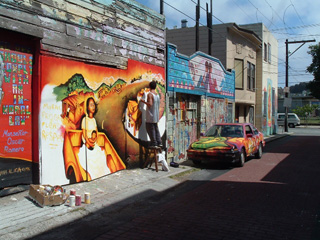
\includegraphics[width=1.85in]{images/mural.jpg}\label{fig:simple.original}}
  \hfil
  \subfigure[{\tt rotate\char`\_180(mural)}]{\includegraphics[width=1.85in]{images/mural_rotate_180.jpg}\label{fig:simple.rotate180}}
  \\
  \subfigure[{\tt rotate\char`\_90\char`\_cw(mural)}]{\hbox{\hspace{0.25in}\includegraphics[height=1.85in]{images/mural_rotate_90_cw.jpg}\hspace{0.25in}\ \label{fig:simple.rotate90cw}}}
  \hfil
  \subfigure[{\tt rotate\char`\_90\char`\_ccw(mural)}]{\hbox{\hspace{0.25in}\includegraphics[height=1.85in]{images/mural_rotate_90_ccw.jpg}\hspace{0.25in}\ \label{fig:simple.rotate90ccw}}}
  \hfil
  \subfigure[{\tt transpose(mural)}]{\includegraphics[height=1.85in]{images/mural_transpose.jpg}\label{fig:simple.transpose}}
  \\
  \subfigure[{\tt flip\char`\_vertical(mural)}]{\includegraphics[width=1.85in]{images/mural_flip_vertical.jpg}\label{fig:simple.flipv}}
  \hfil
  \subfigure[{\tt flip\char`\_horizontal(mural)}]{\includegraphics[width=1.85in]{images/mural_flip_horizontal.jpg}\label{fig:simple.fliph}}
  \\
  \subfigure[{\tt crop(mural,80,60,160,120)}]{\hbox{\hspace{0.5in}\includegraphics[width=0.925in]{images/mural_crop.jpg}\hspace{0.5in}\ \label{fig:simple.crop}}}
  \hfil
  \subfigure[{\tt subsample(mural,2)}]{\hbox{\hspace{0.5in}\includegraphics[width=0.925in]{images/mural_subsample.jpg}\hspace{0.5in}\ \label{fig:simple.subsample}}}
  \\
  \subfigure[{\tt threshold(mural,0.5)}]{\includegraphics[width=1.85in]{images/mural_threshold.jpg}\label{fig:simple.threshold}}
  \hfil
  \subfigure[{\tt clamp(mural,0.25,0.75)}]{\includegraphics[width=1.85in]{images/mural_clamp.jpg}\label{fig:simple.clamp}}
\caption{Sample output from the simple image operations discussed in this section.}
\label{fig:simple}
\end{figure}

The functions listed in the lower section of Table~\ref{tbl:image-manipulation},
on the other hand, all do a small amount of processing of pixel values.
The \verb#pixel_cast()# function converts all the pixels in an image to the
given new pixel type.  The \verb#pixel_cast_rescale()# variants rescale the
values if the channel type has changed, e.g. mapping the 0--255 range of
\verb#uint8# on to the $0.0$--$1.0$ nominal range of \verb#float32#.  The
\verb#channel_*# variants cast the pixels to have the given new channel type,
leaving the overall pixel format unchanged.  The \verb#pixels_to_channels()#
function takes a multi-plane image and reinterprets it as a multi-channel
image with the given pixel type.  Finally, \verb#weighted_rgb_to_gray# converts
RGB pixels to the corresponding grayscale pixel type using an arbitrary
weighting of the red, green, and blue channels.  The default weights are
based on a human perceptual model that weights green most strongly, followed
by red and then blue.

\subsection{Image Algorithms}

\begin{table}[t]\begin{centering}
\begin{tabular}{|c|l|l|} \hline
Function & Description \\ \hline \hline
\verb#copy(im)# & Produce a deep copy of an image \\ \hline
\verb#fill(im,value)# & Fill an image with a pixel value {\it in-place} \\ \hline
\verb#clamp(im,[low],[high])# & Clamp values to the given range \\ \hline
\verb#normalize(im,[low],[high])# & Normalize values to the given range \\ \hline
\verb#threshold(im,[thresh],[low],[high])# & Threshold an image to two values \\ \hline
\verb#grassfire(im)# & Compute the grassfire image of an image \\ \hline
\verb#blob_index(im)# & Apply index numbers to valid regions of an image \\ \hline
\verb#bounding_box(im)# & Return the bounding box of an image \\ \hline
\verb#nonzero_data_bounding_box(im)# & Compute the bounding box of nonzero data \\ \hline
\verb#image_blocks(im,width,height)# & Tile an image with bounding boxes \\ \hline
\end{tabular}
\caption{The simple image algorithms defined in the header file {\tt <vw/Image/Algorithms.h>}.}
\label{tbl:image-algorithms}
\end{centering}\end{table}

We will now introduce a number of additional simple image operations
that are defined in the header file \verb#<vw/Image/Algorithms.h>#.
You have already seen one of them, \verb#copy()#, which forces the
creation of a deep copy of an image in a new buffer.  The rest are
listed in Table~\ref{tbl:image-algorithms}.  The result of two of
these functions can be seen in Figures~\ref{fig:simple.threshold}
and~\ref{fig:simple.clamp}.  We hope to implement a number of
additional image algorithms, mirroring the STL container algorithms
but optimized for images, at some point in the future.

The \verb#fill()# function is noteworthy because it is currently the
only core Vision Workbench function that modifies image data {\it
  in-place}.  It is especially useful for filling a single channel of
an image.  For example, you can use it to make an RGBA image fully
opaque.
\begin{verbatim}
  fill( select_channel( rgba_image, 3 ), 1.0 );
\end{verbatim}
(Note that $1.0$ represents fully-opaque if the image has a
floating-point channel type.)

The \verb#clamp()#, \verb#normalize()#, and \verb#threshold()#
functions return modified versions of their image arguments.
You can assign the result back to the original image, or you can
save it in a different image instead and keep the original.
The \verb#clamp()# function clamps the values in the image to
the given range.  The \verb#normalize# function scales and
shifts the values of an image so that the values span the
specified range.  The default range is from zero to the nominal
maximum value for the channel type, e.g. $1.0$ for floating-point
images.  This is particularly useful for saving intermediate
results of your algorithms to disk for debugging.  Finally, the
\verb#threshold# function returns a two-valued image based on
whether the pixels in the source image is greater than or less
than the given threshold value.  The default high and low output
values are the same as for \verb#norm#, and the default threshold
is zero.  For example, this line will convert a floating-point
grayscale image to pure black-and-white:
\begin{verbatim}
  image = threshold( image, 0.5 );
\end{verbatim}

\begin{figure}[hp]
\centering
  \subfigure[{\tt pattern} (Original)]{
\includegraphics[width=1.85in]{images/pattern.png}\label{fig:complex.original}}
  \hfill
  \subfigure[{\tt normalize( channel\_cast<float>( grassfire(pattern)))}]{\includegraphics[width=1.85in]{images/pattern_grassfire.jpg}\label{fig:complex.grassfire}}
  \hfill
  \subfigure[{\tt normalize( channel\_cast<float>( blob\_index( create\_mask(pattern))))}]{\includegraphics[width=1.85in]{images/pattern_blob_index.jpg}\label{fig:complex.blobindex}}
  \hfill
\caption{Sample output from more complex operations.}
\label{fig:complex}
\end{figure}

The \verb#grassfire()# algorithm, named for the algorithm that
it implements, is more specialized.  It takes an image and
efficiently computes how far each pixel is from from a pixel
whose value is zero, assuming that pixels outside the image
boundaries all have zero value.  It measures distance in the
four-connected Manhattan sense, i.e. as the sum of the
horizontal and vertical distances.  This algorithm is used in
a variety of applications, such as avoiding obstacles and
unknown terrain in path planning.

The \verb#blob_index()# algorithm, applies an index value to isolated
sections of images label valid. The determination of a pixel's
validity is from a special pixel called PixelMask. PixelMask is
discribed in the \emph{Pixels Types} chapter. \verb#blob_index# is
useful algorithm for segmenting an image.


%% The final three functions in this section relate to bounding
%% boxes, which are the topic of the next section.

%% \subsection{Bounding Boxes}

